\section{Защита IPsec на сетевом уровне}
\selectlanguage{russian}

Набор протоколов IPsec (Internet Protocol Security)\index{протокол!IPsec}~\cite{rfc4301} является неотъемлемой частью IPv6\index{протокол!IPv6} и дополнительным необязательным расширением IPv4. IPsec обеспечивает защиту данных на сетевом уровне IP-пакетов.

IPsec определяет:
\begin{itemize}
    \item первичную аутентификацию сторон и управление сеансовыми ключами (протокол IKE, Internet Key Exchange);\index{протокол!IKE}
    \item шифрование с аутентификацией (протокол ESP, Encapsulating Security Payload);\index{протокол!ESP}
    \item только аутентификацию сообщений (протокол AH, Authentication Header).\index{протокол!AH}.
\end{itemize}
Основное (современное) применение этих протоколов состоит в построении VPN\index{протокол!VPN} (Virtual Private Network --- виртуальная частная сеть) при использовании IPsec в так называемом туннельном режиме.

Аутентификация в режимах ESP и AH определяется по-разному. Аутентификация в ESP гарантирует целостность только зашифрованных полезных данных (пакетов следующего уровня после IP). Аутентификация AH гарантирует целостность всего IP-пакета (за исключением полей, изменяемых в процессе передачи пакета по сети).

\subsection{Протокол создания ключей IKE}

%http://www.ietf.org/rfc/rfc4306.txt

Протокол IKE версии 2 (Internet Key Exchange)\index{протокол!IKE}~\cite{rfc4306}, по существу, можно описать следующим образом. Пусть $I$ -- инициатор соединения, $R$ -- отвечающая сторона.

Протокол состоит из двух фаз. Первая фаза очень похожа на установление соединения в SSL/TLS: она включает возможный обмен сертификатами $C_I, C_R$ стандарта X.509 для аутентификации (или альтернативную аутентификацию по общему заранее созданному секретному ключу) и создание общих предварительных сеансовых ключей протокола IKE по протоколу Диффи~---~Хеллмана\index{протокол!Диффи~---~Хеллмана}. Сеансовые ключи протокола IKE служат для шифрования и аутентификации сообщений второй фазы. Вторая фаза создаёт сеансовые ключи для протоколов ESP, AH, то есть ключи для шифрования конечных данных. Сообщения второй фазы также используются для смены ранее созданных сеансовых ключей, и в этом случае протокол сразу начинается со второй фазы с применением ранее созданных сеансовых ключей протокола IKE.

\begin{enumerate}
    \item Создание предварительной защищённой связи для протокола IKE и аутентификация сторон.
        \begin{enumerate}
            \item $I \rightarrow R$: ~ $\left(g^{x_I}\right.$, одноразовая метка $N_I$, идентификаторы поддерживаемых криптографических алгоритмов$\left.\right)$.
                % HDR, SAi1, KEi, Ni   -->

            \item $I \leftarrow R$: ~$\left(g^{x_R}\right.$, одноразовая метка $N_R$, идентификаторы выбранных алгоритмов, запрос сертификата $C_I\left.\right)$.
                % <--    HDR, SAr1, KEr, Nr, [CERTREQ]

                Протокол Диффи~---~Хеллмана\index{протокол!Диффи~---~Хеллмана} оперирует с генератором $g=2$ в группе $\Z_p^*$ для одного из двух фиксированных $p$ длиной 768 или 1024 бита. После обмена элементами $g^{x_I}$ и $g^{x_R}$ обе стороны обладают общим секретом $g^{x_I x_R}$.

                Одноразовые метки $N_I, N_R$ созданы криптографическим генератором псевдослучайных чисел $PRF$.

                После данного сообщения стороны договорились об используемых алгоритмах и создали общие сеансовые ключи:
                    \[ seed = PRF(N_i ~\|~ N_r, ~g^{x_I x_R}), \]
                    \[ \{ K_d \| Ka_I \| Ka_R \| Ke_I \| Ke_R
                        % \| Kp_I \| Kp_R
                        \} = PRF(seed, ~ N_i ~\|~ N_r), \]
                где $Ka_I, Ka_R$ -- ключи кода аутентификации для связи в оба направления, ~ $Ke_I, Ke_R$ -- ключи шифрования сообщений для двух направлений, ~ $K_d$ -- инициирующее значение генератора $PRF$ для создания сеансовых ключей окончательной защищённой связи, ~ функцией $PRF(x)$ обозначается выход генератора с инициализирующим значением $x$.
                %$Kp_I, Kp_R$ --  which areused when generating an AUTH payload.

                Дальнейший обмен данными зашифрован алгоритмом AES в режиме CBC со случайно выбранным инициализирующим вектором $IV$ на сеансовых ключах $Ke$ и аутентифицирован имитовставкой\index{имитовставка} на ключах $Ka$. Введём обозначения для шифрования сообщения $m$ со сцеплением блоков $E_{Ke_X}(m)$ и совместного шифрования и добавления кода аутентификации сообщений $\langle m \rangle_X$ для исходящих данных от стороны $X$:
                    \[  E_{Ke_X}(m) = IV ~\|~ E_{Ke_X}(IV ~\|~ m), \]
                    \[  \langle m \rangle_X = E_{Ke_X}(m) ~\|~ \HMAC(Ka_X, ~ E_{Ke_X}(m)). \]

            \item $I \rightarrow R$: ~ $\langle ID_I, ~ C_I, ~\text{запрос сертификата}~ C_R, ~ ID_R, ~ A_I \rangle_I$.
                % HDR, SK {IDi, [CERT,] [CERTREQ,] [IDr,] AUTH, SAi2, TSi, TSr}     -->

                По значениям идентификаторов $ID_I, ID_R$ сторона $R$ проверяет знание стороной $I$ ключей $Ke, Ka$.

                Поле $A_I$ обеспечивает аутентификацию стороны $I$ стороне $R$ по одному из двух способов. Если используются сертификаты, то $I$ показывает, что обладает закрытым ключом, парным открытому ключу сертификата $C_I$, подписывая сообщение $data$:
                    \[ A_I = \textrm{ЭП}(data). \]
                Сторона $R$ также проверяет сертификат $C_I$ по цепочке до доверенного сертификата верхнего уровня.

                Второй вариант аутентификации -- по общему секретному симметричному ключу аутентификации $K_{IR}$, который заранее был создан $I$ и $R$, как в Kerberos. Сторона $I$ показывает, что знает общий секрет, вычисляя
                    \[ A_I = PRF( PRF(K_{IR}, ~ \text{текст ''Key Pad for IKEv2''}), ~ data). \]
                Сторона $R$ сравнивает присланное значение $A_I$ с вычисленным и убеждается, что $I$ знает общий секрет.

                Сообщение $data$ -- это открытое сообщение данной транзакции, за исключением нескольких полей.

            \item $I \leftarrow R$: ~ $\langle ID_R, ~ C_R, ~ A_R \rangle_R$.
                % HDR, SK {IDr, [CERT,] AUTH, SAr2, TSi, TSr}

                Производится аутентификация стороны $R$ стороной $I$ аналогичным образом.
        \end{enumerate}

    \item Создание защищённой связи для протоколов ESP, AH, то есть ключей шифрования и кодов аутентификации конечных полезных данных. Фаза повторяет первые две транзакции первой фазы с созданием ключей по одноразовой метке $N'$ и протоколу Диффи~---~Хеллмана\index{протокол!Диффи~---~Хеллмана} с секретными ключами $x'$.
        \begin{enumerate}
            \item $I \rightarrow R$: ~ $\langle g^{x'_I}$, одноразовая метка $N'_I$, поддерживаемые алгоритмы для ESP, AH$\rangle_I$.
                % HDR, SK {[N], SA, Ni, [KEi], [TSi, TSr]}             -->
            \item $I \rightarrow R$: ~ $\langle g^{x'_R}$, одноразовая метка $N'_R$, выбранные алгоритмы для ESP, AH$\rangle_R$.
                % <--    HDR, SK {SA, Nr, [KEr], [TSi, TSr]}
        \end{enumerate}
        По окончании второй фазы обе стороны имеют общие секретные ключи $Ke, Ka$ для шифрования и кодов аутентификации в двух направлениях, от стороны $I$ и от стороны $R$:
            \[ \{Ka'_I ~\|~ Ka'_R ~\|~ Ke'_I ~\|~ Ke'_R \} = PRF(K_d, ~ g^{x'_I x'_R} ~\|~ N'_I ~\|~ N'_r). \]
\end{enumerate}

Итогом протокола IKE является набор сеансовых ключей для шифрования $Ke'_I, ~ Ke'_R$ и кодов аутентификации $Ka'_I, ~ Ka'_R$ в протоколах ESP и AH.


\subsection{Таблица защищённых связей}

\textbf{Защищённая связь} (Security Association, SA) является \emph{однонаправленной} от отправителя к получателю и характеризуется тремя основными параметрами:
\begin{itemize}
    \item индексом параметров защиты -- уникальное 32-битовое число, входит в заголовок ESP- и AH- пакетов;
    \item IP-адресом стороны-отправителя;
    \item идентификатором применения ESP- или AH-протокола.
\end{itemize}

Защищённые связи хранятся в таблице защищённых связей со следующими полями:
\begin{itemize}
    \item счётчик порядкового номера, входит в заголовок ESP- и AH-пакетов,
    \item окно защиты от воспроизведения -- скользящий буфер порядковых номеров пакетов для защиты от пропуска и повтора пакетов,
    \item информация протокола ESP и AH -- алгоритмы, ключи, время действия ключей,
    \item режим протокола: транспортный или туннельный.
\end{itemize}

По индексу параметров защиты, находящемся в заголовке ESP- и AH-пакетов, получатель из таблицы защищённых связей извлекает параметры (названия алгоритмов, ключи и т.~д.), производит проверки счётчиков, аутентифицирует и расшифровывает вложенные данные для принятого IP-пакета.
%Или создаёт зашифрованный аутентифицированный IP-пакет, который включает индекс параметров защиты, чтобы получатель мог из своей таблицы защищённых связей извлечь ключи для аутентификации и расшифрования.

Протоколы ESP и AH можно применять к IP-пакету в трёх вариантах:
\begin{itemize}
    \item только ESP-протокол;
     \item только AH-протокол;
    \item последовательное применение ESP и AH протоколов.
\end{itemize}
Подчеркнём, что только AH-протокол гарантирует целостность всего IP-пакета, поэтому для организации виртуальной сети VPN\index{сеть!виртуальная частная}, как правило, применяется третий вариант (последовательно ESP и AH протоколы).


\subsection{Транспортный и туннельный режимы}

Протоколы ESP, AH могут применяться в транспортном режиме, когда исходный IP-пакет расширяется заголовками и концевиками протоколов ESP, AH, или в туннельном режиме, когда весь IP-пакет вкладывается в новый IP-пакет, который включает заголовки и концевики ESP, AH.

Новый IP-пакет в туннельном режиме может иметь другие IP-адреса, отличные от оригинальных. Именно это свойство используется для построения виртуальных частных сетей (Virtual Private Network, VPN)\index{сеть!виртуальная частная}. IP-адресом нового пакета является IP-адрес IPsec шлюза виртуальной сети. IP-адрес вложенного пакета является локальным адресом виртуальной сети. IPsec шлюз производит преобразование IPsec пакетов в обычные IP-пакеты виртуальной сети и наоборот.

Схемы транспортного и туннельного режимов показаны ниже отдельно для ESP- и AH-протоколов.


\subsection{Протокол шифрования и аутентификации ESP}

Протокол ESP\index{протокол!ESP} определяет шифрование и аутентификацию вложенных в IP-пакет сообщений в формате, показанном на рис.~\ref{fig:ipsec-esp}.

\begin{figure}[!ht]
	\centering
	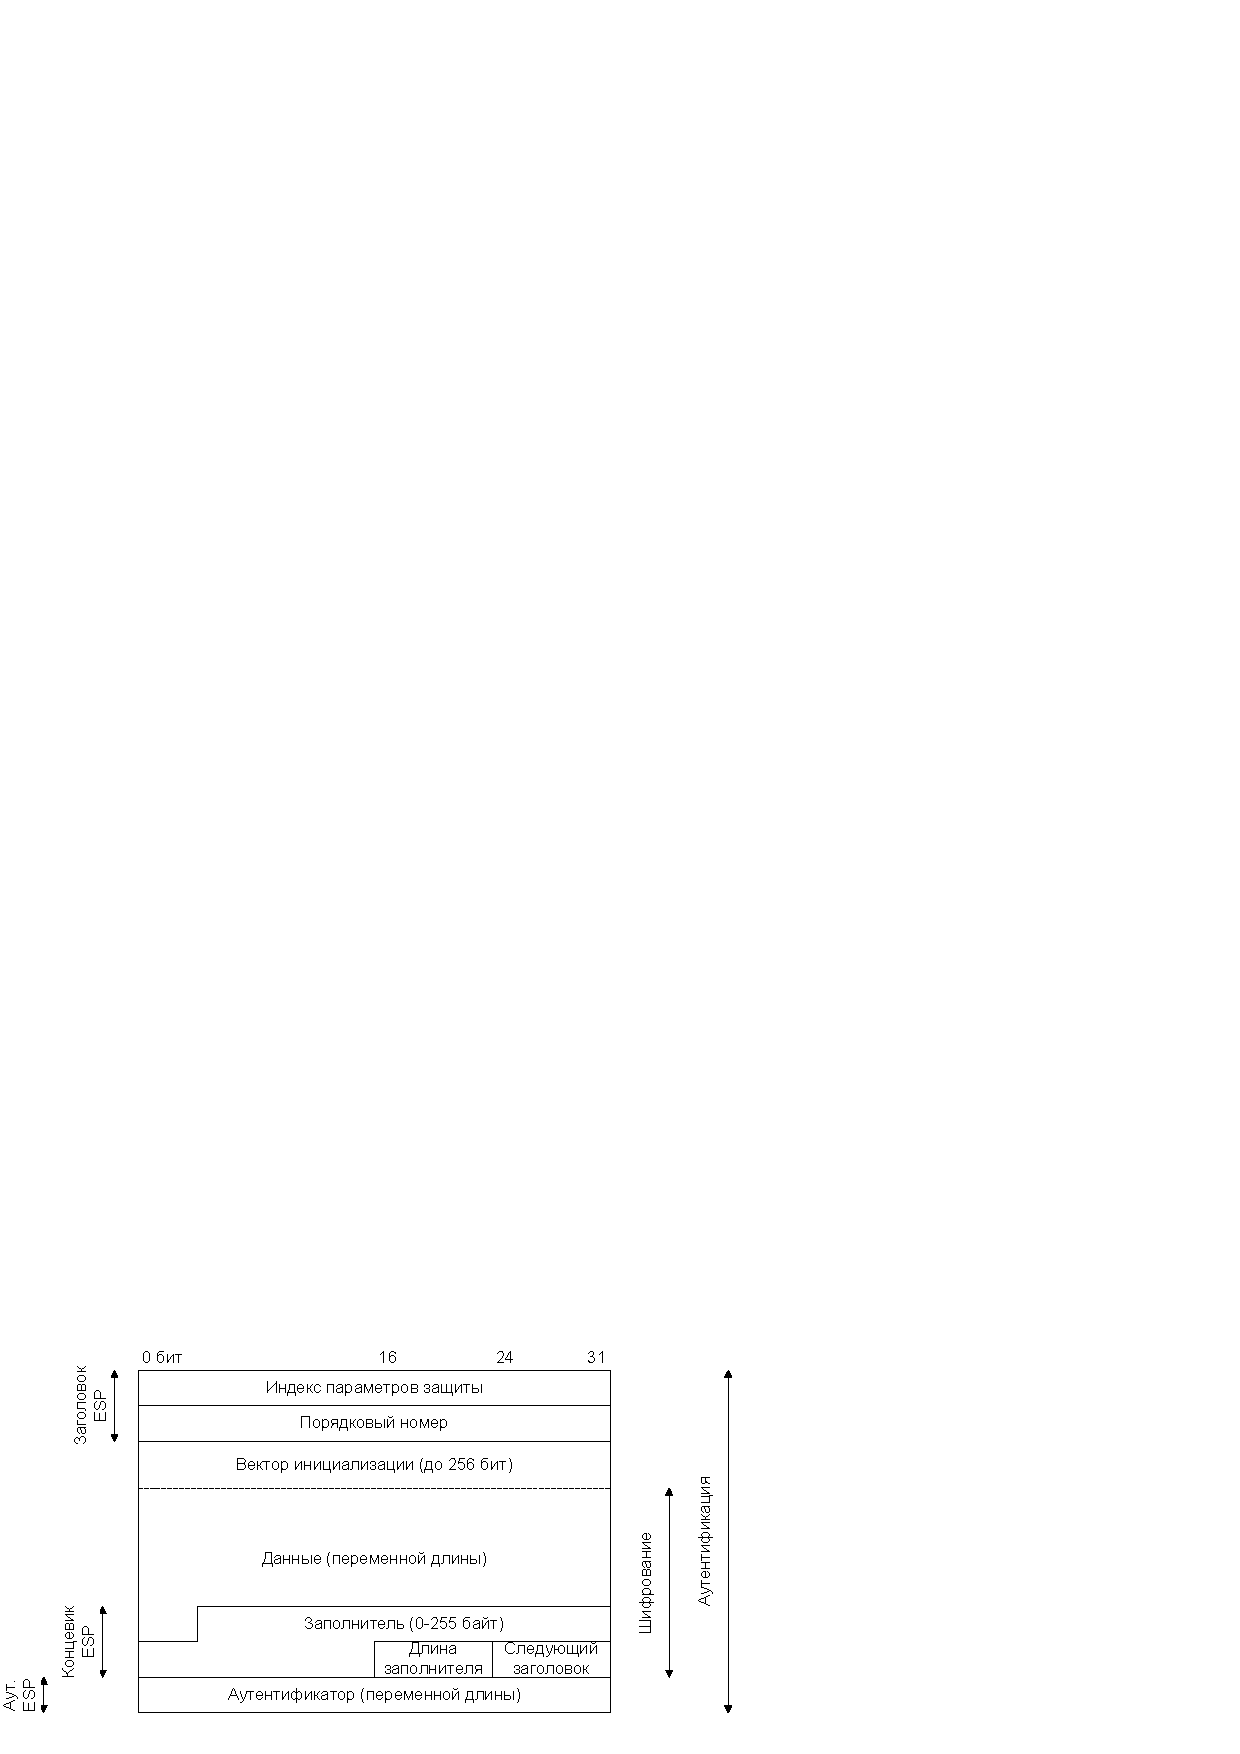
\includegraphics[width=0.9\textwidth]{pic/ipsec-esp}
	\caption{Формат ESP пакета\label{fig:ipsec-esp}}
\end{figure}

Шифрование вложенных данных производится в режиме CBC алгоритмом AES на ключе $Ke'$ с псевдослучайным вектором инициализации IV, вставленном перед зашифрованными данными.

Аутентификатор сообщения определяется как усечённое до 96 бит значение $\HMAC(Ka', m)$, вычисленное стандартным способом.

\begin{figure}[!ht]
	\centering
	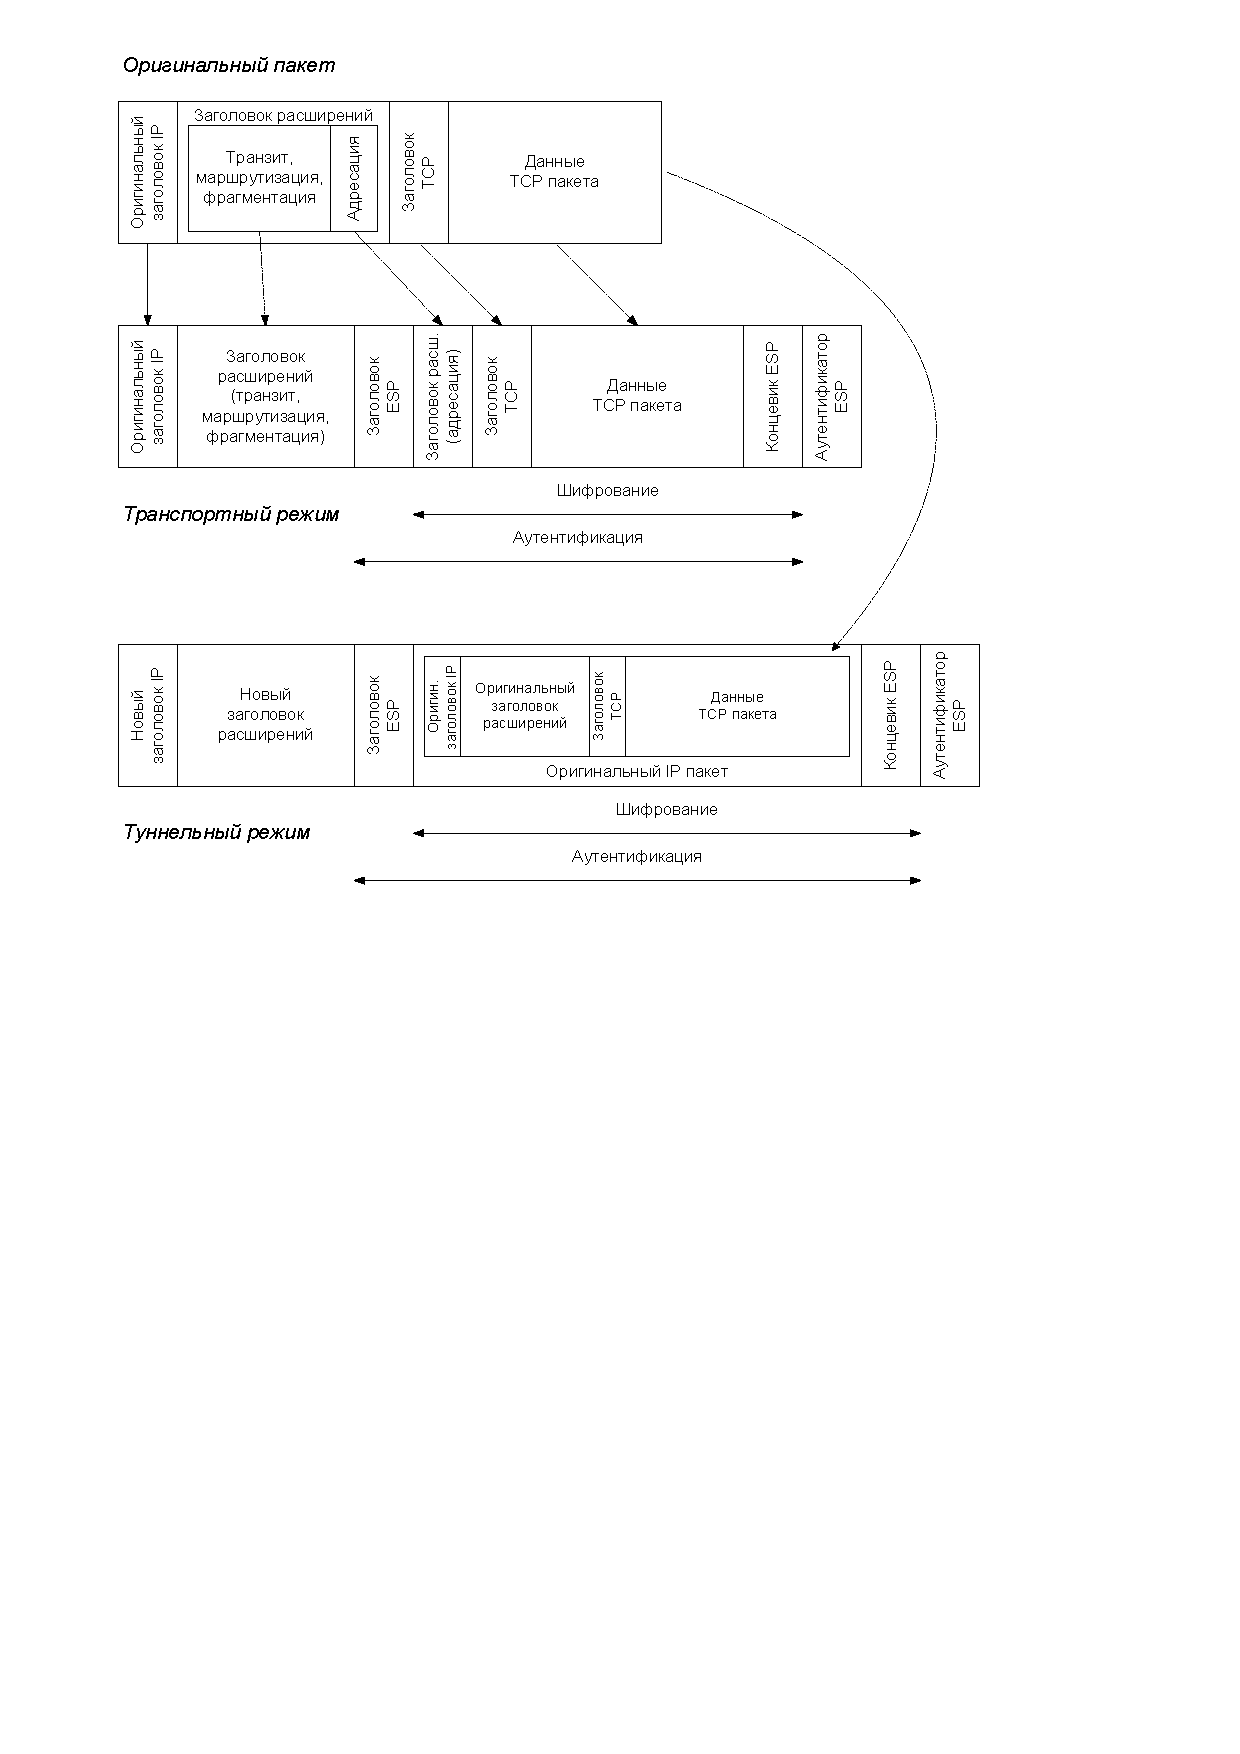
\includegraphics[width=0.9\textwidth]{pic/ipsec-esp-modes}
	\caption{Применение ESP протокола к пакету IPv6\label{fig:ipsec-esp-modes}}
\end{figure}

На рис.~\ref{fig:ipsec-esp-modes} показано применение протокола в транспортном и туннельном режимах.


\subsection{Протокол аутентификации AH}

Протокол AH определяет аутентификацию всего IP-пакета в формате, показанном на рис.~\ref{fig:ipsec-ah}.

\begin{figure}[!ht]
	\centering
	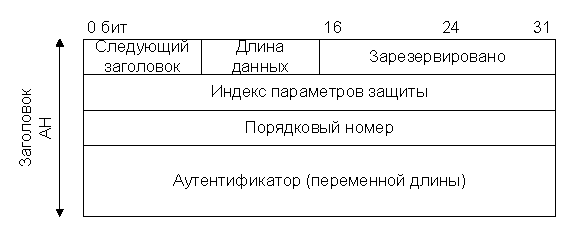
\includegraphics[width=0.7\textwidth]{pic/ipsec-ah}
	\caption{Заголовок AH пакета\label{fig:ipsec-ah}}
\end{figure}

Аутентификатор сообщения определяется так же, как и в протоколе ESP -- усечённое до 96 бит значение $\HMAC(Ka', m)$, вычисленное стандартным способом.

\begin{figure}[!ht]
	\centering
	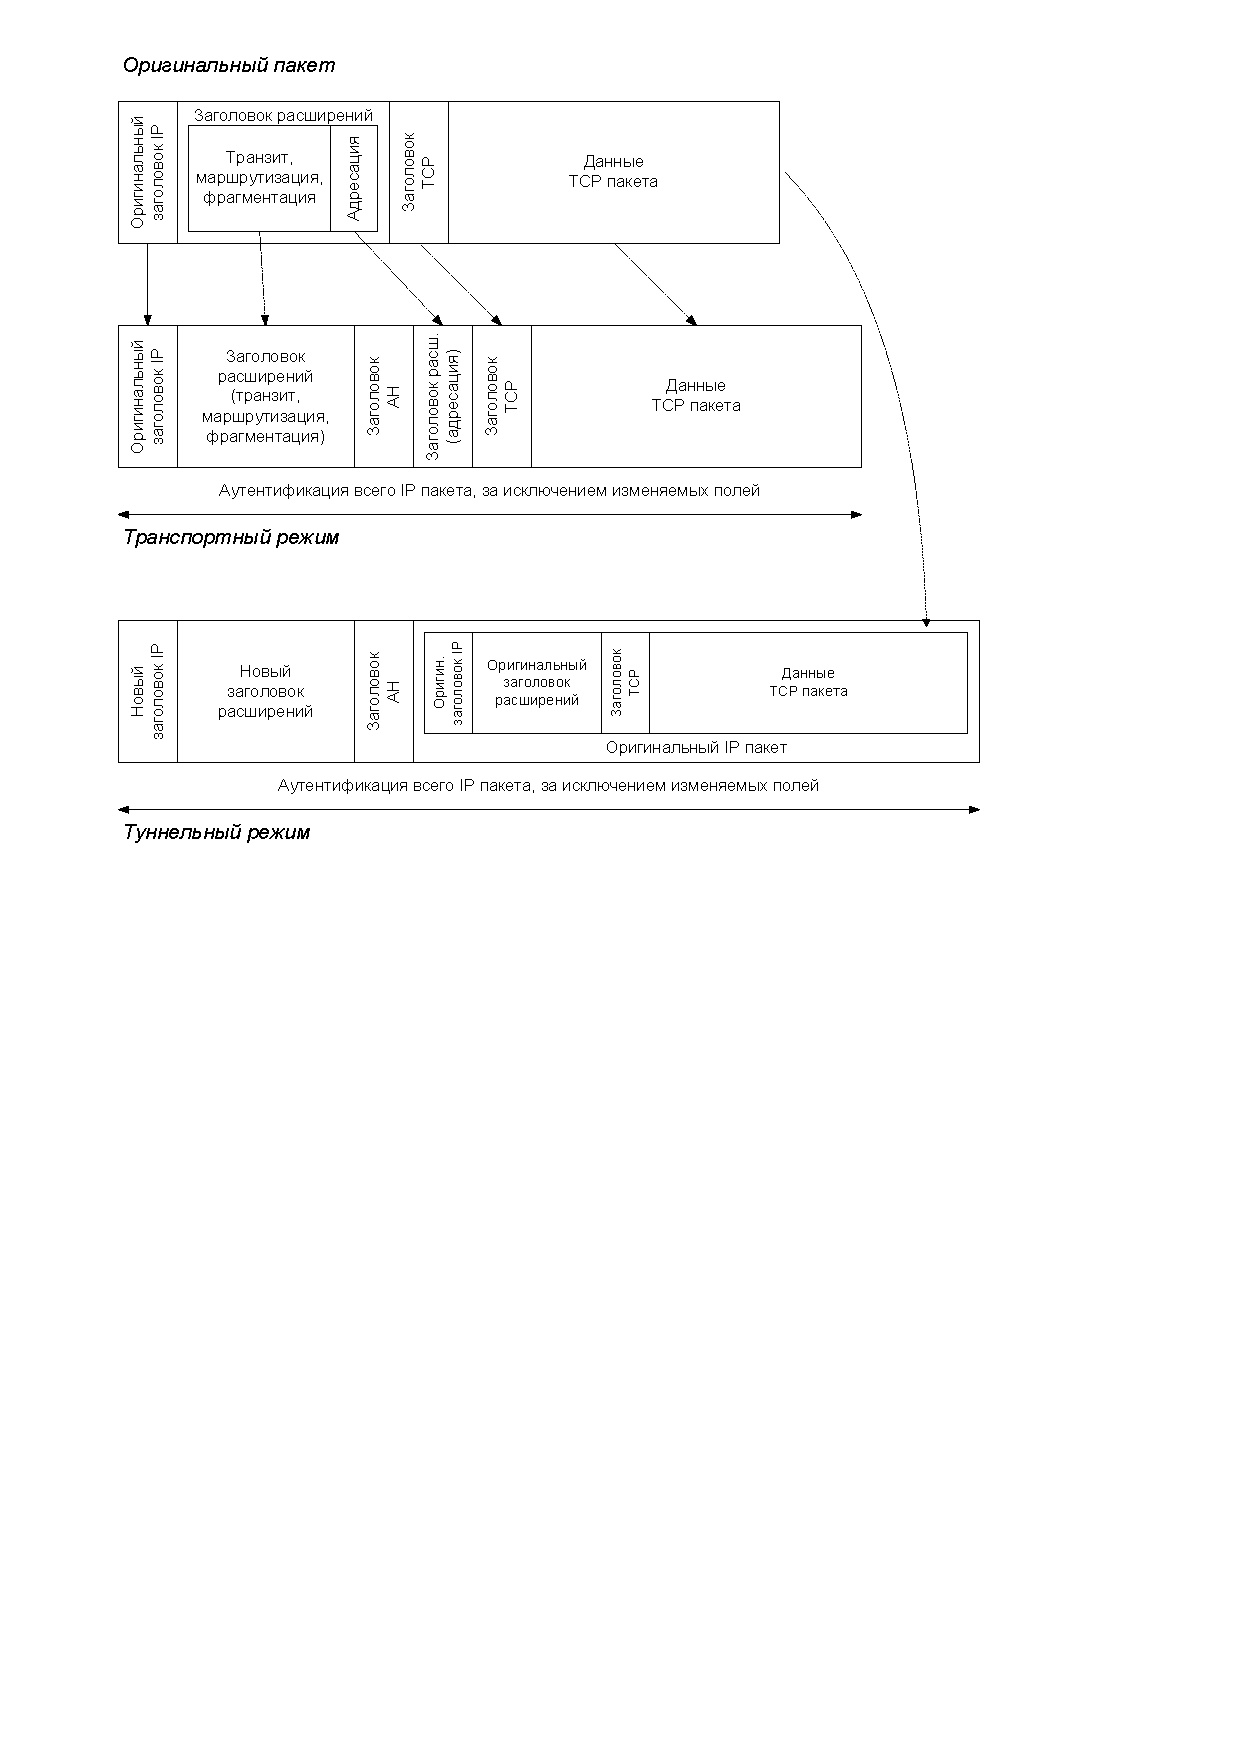
\includegraphics[width=0.9\textwidth]{pic/ipsec-ah-modes}
	\caption{Применение протокола AH к пакету IPv6\label{fig:ipsec-ah-modes}}
\end{figure}

На рис.~\ref{fig:ipsec-ah-modes} показано применение протокола в транспортном и туннельном режимах.
